\documentclass[pdflatex,sn-mathphys-num]{sn-jnl}

\usepackage[T1]{fontenc}
\usepackage{amsmath,amssymb}
\usepackage{float}
\floatstyle{ruled}
\newfloat{algorithm}{tbp}{loa}
\floatname{algorithm}{Algorithm}
\usepackage{algpseudocode}
\algrenewcommand\algorithmicrequire{\textbf{Input:}}
\algrenewcommand\algorithmicensure{\textbf{Output:}}
\usepackage{booktabs}
\usepackage{array}
\usepackage{graphicx}
\usepackage{tikz}
\usepackage{pgfplots}
\pgfplotsset{compat=1.17}
\usetikzlibrary{arrows.meta,calc,positioning}
\hypersetup{hypertexnames=false}

\newcommand{\ci}[3]{\begin{tabular}[c]{@{}c@{}}$#1$\\{}[$#2$, $#3$]\end{tabular}}
\newcommand{\cib}[3]{{\boldmath\ci{#1}{#2}{#3}}}
\newcommand{\cit}[3]{\begin{tabular}[t]{@{}c@{}}$#1$\\{}[$#2$, $#3$]\end{tabular}}
\newcommand{\cibt}[3]{{\boldmath\cit{#1}{#2}{#3}}}
\newcommand{\scl}{SCL}
\newcommand{\aob}{AOB}
\newcommand{\twol}[2]{\begin{tabular}[c]{@{}l@{}}#1\\#2\end{tabular}}

\raggedbottom
\renewcommand{\topfraction}{0.85}
\renewcommand{\bottomfraction}{0.6}
\renewcommand{\textfraction}{0.12}
\renewcommand{\floatpagefraction}{0.75}
\setcounter{topnumber}{3}
\setcounter{totalnumber}{5}
% e-mail list without a trailing separator (as in the earlier versions)
\makeatletter
\def\email#1{\global\advance\emailcnt by 1\relax
\if@corauemail
  \ifx\corrauthemail\@empty\g@addto@macro\corrauthemail{\textcolor{blue}{#1}}%
  \else\g@addto@macro\corrauthemail{;\ \textcolor{blue}{#1}}\fi
\else
  \ifx\authemail\@empty\g@addto@macro\authemail{\textcolor{blue}{#1}}%
  \else\g@addto@macro\authemail{;\ \textcolor{blue}{#1}}\fi
\fi}
\makeatother

\begin{document}

\title[Self-Calibrating Control Layer for Multi-Object Trackers]{Training-Free Self-Calibrating Control Layer for Heterogeneous Multi-Object Trackers}

\author*[1]{\fnm{Ahmed Gouda} \sur{Ismail}}\email{a7medgouda1@gmail.com}
\author[1]{\fnm{Mohamed S.} \sur{Mohamed}}\email{mohamedms@mtc.edu.eg}
\author[2]{\fnm{Tarek Ahmed} \sur{Mahmoud}}\email{tarek.mohamed@eui.edu.eg}

\affil*[1]{\orgdiv{Computer Engineering and Artificial Intelligence Department}, \orgname{Military Technical College}, \orgaddress{\city{Cairo}, \country{Egypt}}}
\affil[2]{\orgdiv{Computer Engineering Department}, \orgname{Egypt University of Informatics}, \orgaddress{\city{Cairo}, \country{Egypt}}}

\abstract{Many multi-object tracking systems combine a detector and a tracker developed separately. When the detector is replaced, retrained, or quantized, its confidence scores change, but the tracker keeps thresholds set for another detector. This paper presents a training-free self-calibrating control layer (SCL) between a frozen detector and a frozen tracker. It splits the detector scores of recent frames with Otsu's histogram threshold and decides whether the stream is clean or noisy. On clean streams it keeps the tracker's settings; on noisy streams it chooses which candidates reach the tracker, assigns them new scores, and sets the tracker's thresholds. It also adds a continuation step for trackers that lack one. It needs no labels and no future frames. One frozen configuration was evaluated with nine published trackers on MOT17, KITTI, and DanceTrack. It raised the higher order tracking accuracy (HOTA) of two single-stage trackers by 0.9\%: OC-SORT, used during development, and PD-SORT, which was not. When all detector scores were halved, two trackers failed completely; with \scl{}, both recovered at least 97\% of their original HOTA. With a noisy RT-DETR-L detector, it raised the multiple object tracking accuracy (MOTA) of ByteTrack and BoT-SORT by 12.6\% and 16.3\%. Five two-stage trackers with well-matched detections changed by less than 0.1\% in HOTA. In failure cases, it lowered the HOTA of C-TWiX on KITTI cars by 1.7\% and the MOTA of two two-stage trackers with a YOLOv8n detector by up to 4.9\%. It adds 2.95 ms per frame on a central processing unit.}

\keywords{Multi-object tracking, Tracking by detection, Detector confidence, Online adaptation, Otsu thresholding, Video analysis}

\maketitle

\section{Introduction}\label{sec:intro}

Multi-object tracking (MOT) finds every object of interest in a video and
gives each object the same identity over time. It is used in surveillance,
driving, and drone systems
\cite{zhu2022visdrone,wu2022uavsurvey,lu2024uavdetection}, and many of these
systems must give results with little delay. Most trackers follow the
tracking-by-detection design. A detector gives a score to each candidate box
in a frame, and the tracker links the boxes whose scores pass its thresholds
into tracks \cite{bewley2016sort,zhang2022bytetrack,cao2023ocsort}.

In real systems, the detector and the tracker are rarely built together. A
detector is replaced by a faster model, retrained for a new camera, or made
smaller (quantized) for embedded hardware. The tracker, however, keeps the
thresholds that its authors set for another detector. Detector scores are not
calibrated across models and conditions \cite{kuppers2020detcalib}, so a new
detector usually gives scores on a different scale, and nothing in the system
notices the change.

The effect can be large. In this paper, halving the scores of a published
detector reduces two well-known trackers to 0 higher order tracking accuracy
(HOTA) \cite{luiten2021hota}, because no detection passes their fixed
thresholds (Sect.~\ref{sec:shift}). Retuning every tracker for every detector
needs labelled data from the new setting, which a working system usually does
not have.

Current methods solve only part of this problem. Trackers with adaptive
thresholds change their own thresholds from the detections of each frame, but
each method is built into one tracker
\cite{ma2023adaptivebytetrack,shim2024adaptrack,act2026adaptive}. Score
calibration methods correct the detector scores, but they need labelled data
\cite{kuppers2020detcalib}. Adaptive inference methods learn or measure a
policy for one model \cite{han2022dynamic,jiang2018chameleon}. What is missing
is a component that needs no training, works outside the tracker, adjusts itself
from the detector's own scores, and leaves the tracker alone when it already
fits those scores.

This paper presents such a component: a self-calibrating control layer (\scl{})
that sits between a fixed (frozen) detector and a fixed tracker. It reads the
detector scores and the settings that the tracker declares, and it decides
while running whether the tracker needs help. The main idea is simple: the
detector's own scores show whether its output fits the tracker. \scl{} looks
at the scores of recent frames and checks how clearly they separate confident
objects from clutter. If the separation is clear, the tracker keeps its own
settings, and the layer only adds help that the tracker lacks, such as a step
that continues tracks. If it is not clear, \scl{} chooses which candidates
reach the tracker, assigns them new scores, and sets the tracker's thresholds.
The novelty is therefore a layer outside the tracker that needs no labels,
uses one fixed configuration for many trackers, and stays out of the way when
the tracker already fits the detector.

The main contributions are:
\begin{enumerate}
\item \scl{}, a control layer that needs no training, adjusts itself from the
      detector scores, uses no future frames, keeps the tracker's settings
      when the scores are clean, and takes full control only when they are
      noisy (Sect.~\ref{sec:method}).
\item A host contract, a set of four numbers from the tracker's published
      settings, that lets one fixed configuration work with single-stage and
      two-stage trackers without changing them (Sect.~\ref{sec:contract}).
\item A development path from always-on banding (\aob{}), an earlier design
      that always intervened, in which each step is compared with that
      baseline (Sect.~\ref{sec:development}).
\item A test of one fixed configuration on nine published trackers and three
      datasets, with development data and two groups of external systems
      that were declared before they were run, paired bootstrap intervals,
      the failure cases, and a speed measurement on a central processing
      unit (CPU) (Sects.~\ref{sec:setup} to~\ref{sec:discussion}).
\end{enumerate}

The rest of the paper is organized as follows. Section~\ref{sec:data-eval}
describes the data, the evaluation roles, and the metrics, and
Section~\ref{sec:related} reviews related work. Section~\ref{sec:method}
explains \scl{} and all its settings, and Section~\ref{sec:development} shows
how it was developed from an earlier design that always intervened. The
configuration was then frozen before any external system was run.
Section~\ref{sec:setup} gives the experimental setup,
Section~\ref{sec:results} the results, Section~\ref{sec:discussion} their
analysis and the limitations, and Section~\ref{sec:conclusion} concludes the
paper.

\section{Data and Evaluation}\label{sec:data-eval}

\subsection{Detectors and data}\label{sec:data}
Table~\ref{tab:data} lists the evaluation cells. A cell is one combination of
data, detector, and tracker (the trackers are introduced in
Sect.~\ref{sec:setup}). On MOT17 val-half \cite{milan2016mot16} the trackers
use the published YOLOX-X detections \cite{ge2021yolox}. The emission floor is
the lowest detector score that is passed on; it is 0.01 or 0.1
(Table~\ref{tab:mot17}). On KITTI tracking training \cite{geiger2012kitti},
the trackers run with two detectors that differ from the MOT17 detector:
YOLOv8n \cite{jocher2023yolov8} and RT-DETR-L \cite{zhao2024rtdetr}. To study
the score problem directly, the published MOT17 scores were also changed
before the tracker by four monotone transforms: cubing ($s^3$), halving ($0.5\,s$),
and logit temperatures $T=2$ and $T=0.5$, $\sigma(z/T)$. A temperature
divides the logit $z$ of each score by $T$ before turning it back into a
score: $T=2$ pulls all scores toward 0.5, and $T=0.5$ pushes them toward 0
and 1. The trackers kept their published thresholds. During development,
the layer was also run with ByteTrack on aerial video: the seven sequences of
VisDrone2019-MOT val \cite{zhu2022visdrone} and 40 sequences of its training
set, with YOLOv8n, RT-DETR-L, and (on val) Faster R-CNN detections. These runs
used a class-agnostic protocol and served only to understand the mechanisms;
the same seven val sequences are the evaluation set of our earlier work on
detector-side control (Sect.~\ref{sec:related}). The external systems use the
detections released by their authors: on MOT17 val-half, on the KITTI
tracking sequences of the KITTI MOTS validation split, and on DanceTrack val
\cite{sun2022dancetrack}.

\begin{table*}[t]
\caption{Evaluation cells and their role. Development cells were visible while
the layer was designed. External cells were declared before they were run and
were run once with the frozen configuration: PD-SORT and Hybrid-SORT in the
freeze commit, the others under a protocol registered after the freeze and
before any run.}
\label{tab:data}
\centering\footnotesize
\setlength{\tabcolsep}{3pt}
\begin{tabular}{@{}>{\raggedright\arraybackslash}p{31mm}>{\raggedright\arraybackslash}p{28mm}>{\raggedright\arraybackslash}p{35mm}>{\raggedright\arraybackslash}p{26mm}@{}}
\toprule
Data & Detector & Trackers & Role\\
\midrule
MOT17 val-half (7 sequences) & published YOLOX-X detections & ByteTrack (2 settings), OC-SORT, BoostTrack, SparseTrack & development\\
KITTI tracking training (21 sequences) & RT-DETR-L; YOLOv8n & ByteTrack, BoT-SORT, OC-SORT (each with both detectors) & development (detector change)\\
MOT17 val-half, score transforms & published YOLOX-X, transformed scores & ByteTrack (2 settings), OC-SORT, BoostTrack & development (robustness)\\
VisDrone2019-MOT val (7) and train (40 sequences) & YOLOv8n, RT-DETR-L, Faster R-CNN & ByteTrack & development (aerial video, mechanisms only)\\
MOT17 val-half & released PD-SORT / Hybrid-SORT detections & PD-SORT, Hybrid-SORT & external, declared at the freeze\\
MOT17 val-half; KITTI MOTS val (9 sequences); DanceTrack val (25) & detections released by the authors & C-TWiX & external, declared after the freeze\\
DanceTrack val (25 sequences) & detections released by the authors & TrackTrack & external, declared after the freeze\\
MOT17 val-half & authors' detector & TOPICTrack & external; reproduction FAILED, excluded\\
\bottomrule
\end{tabular}
\end{table*}


\subsection{Evaluation roles and metrics}\label{sec:roles}
Every cell has one of three roles (Table~\ref{tab:data}). Development cells
were visible while \scl{} was designed: MOT17 with four trackers, KITTI with
three trackers and two other detectors, the score transforms, and the VisDrone
runs. Their gains are measured, but they are not held-out evidence. The
external systems were never used during design. Two of them, PD-SORT and
Hybrid-SORT, were chosen and declared in the commit that froze the
configuration. Three more recent systems, C-TWiX, TOPICTrack, and TrackTrack,
were chosen after the freeze under a protocol that was registered before any
run. It fixed the selection criteria, the host contracts, the reproduction
classes, and a prediction of the layer's effect for each system, and it
required every system that met the criteria to be reported, whatever the
result. Each external system was run once with the frozen configuration. For
each external tracker, our reproduction is compared with the authors' number
and marked EXACT (within 0.2 HOTA), CLOSE (within 1.0 HOTA, with a documented
cause that was not tuned), or FAILED; a system with a FAILED reproduction is
excluded from the analysis.

\label{sec:metrics}Table~\ref{tab:metrics} gives the three tracking metrics,
HOTA, multiple object tracking accuracy (MOTA), and identity F1 score (IDF1),
and their definitions. They are built from three error counts: false
positives (FP), missed objects or false negatives (FN), and identity switches
(IDS). They are computed with the TrackEval library (commit
12c8791) and the official ground truth of each benchmark, following
MOTChallenge practice \cite{dendorfer2021motchallenge}. On KITTI tracking
with our two detectors, HOTA is the official value averaged over cars and
pedestrians; for C-TWiX, cars and pedestrians are reported separately, as in
the authors' evaluation.

\begin{table*}[t]
\caption{Tracking metrics used in this paper. GT is the number of
ground-truth boxes; FP, FN, and IDS are the false positives, missed objects
(false negatives), and identity switches, summed over all frames. For IDF1,
each ground-truth track is first matched to at most one output track, and
IDTP, IDFP, and IDFN are the true-positive, false-positive, and
false-negative boxes under this matching. For HOTA, at a localization
threshold $\alpha$, $\mathrm{TP}_\alpha$, $\mathrm{FN}_\alpha$, and
$\mathrm{FP}_\alpha$ are the matched, missed, and unmatched boxes, and
$\mathcal{A}(c)$ is the association accuracy of a matched pair $c$. HOTA,
MOTA, and IDF1 are given in percent.}
\label{tab:metrics}
\centering\footnotesize
\setlength{\tabcolsep}{4pt}
\renewcommand{\arraystretch}{1.6}
\begin{tabular}{@{}l>{\raggedright\arraybackslash}p{68mm}>{\raggedright\arraybackslash}p{40mm}@{}}
\toprule
Metric & Definition & What it measures\\
\midrule
MOTA \cite{bernardin2008clear} & $\displaystyle \mathrm{MOTA}=1-\frac{\mathrm{FN}+\mathrm{FP}+\mathrm{IDS}}{\mathrm{GT}}$ & overall error count; reacts strongly to false positives and missed objects\\
IDF1 \cite{ristani2016idf1} & $\displaystyle \mathrm{IDF1}=\frac{2\,\mathrm{IDTP}}{2\,\mathrm{IDTP}+\mathrm{IDFP}+\mathrm{IDFN}}$ & how long each object keeps the correct identity\\
HOTA \cite{luiten2021hota} & $\displaystyle \mathrm{HOTA}=\frac{1}{19}\sum_{\alpha}\sqrt{\mathrm{DetA}_\alpha\,\mathrm{AssA}_\alpha}$,\newline $\displaystyle \mathrm{DetA}_\alpha=\frac{|\mathrm{TP}_\alpha|}{|\mathrm{TP}_\alpha|+|\mathrm{FN}_\alpha|+|\mathrm{FP}_\alpha|}$,\newline $\displaystyle \mathrm{AssA}_\alpha=\frac{1}{|\mathrm{TP}_\alpha|}\sum_{c\in\mathrm{TP}_\alpha}\mathcal{A}(c)$,\newline with $\alpha=0.05,0.10,\dots,0.95$ & balance of detection (DetA) and association (AssA); the main metric of this paper\\
\bottomrule
\end{tabular}
\end{table*}


All comparisons are paired: each tracker runs with and without \scl{} on
the same sequences. Differences are pooled over sequences, and their 95\%
intervals come from a percentile bootstrap over sequences
\cite{efron1993bootstrap} with 10,000 resamples and seed 42. A difference is
called significant when its interval does not include zero. The intervals
are computed for each comparison separately, without a correction for
multiple comparisons. As a simple
check that does not depend on any distribution, we also count the sequences
where HOTA rose, stayed the same ($|\Delta\mathrm{HOTA}|<0.01$), or fell.

HOTA, MOTA, and IDF1 are given in percent, and higher values are better. FP,
FN, and IDS are counts, and lower values are better. Runtime is given in
milliseconds (ms) per frame, and lower values are better.

\section{Related Work}\label{sec:related}

\scl{} is related to four lines of research: the trackers it works with, the
confidence of the detectors that feed them, trackers that adapt their own
thresholds, and methods that adapt inference while running. They are
reviewed below in this order, and Table~\ref{tab:related} compares the
closest methods with \scl{}.

Most practical trackers follow the tracking-by-detection design. SORT
predicts each box with a Kalman filter and matches the predictions to new
detections by overlap with the Hungarian method \cite{bewley2016sort}.
ByteTrack added a second matching step that uses low-score detections to
continue existing tracks \cite{zhang2022bytetrack}, and many later trackers
kept this two-stage design. Others, such as OC-SORT \cite{cao2023ocsort}, use
only one score threshold. Recent designs learn association from box
coordinates (C-TWiX \cite{miah2025twix}), run parallel association paths
(TOPICTrack \cite{cao2025topictrack}), or focus association on tracks with
two views of the detections (TrackTrack \cite{shim2025tracktrack}). All these
trackers read detector scores through fixed thresholds that were tuned for one
detector, usually YOLOX \cite{ge2021yolox}. Nine published trackers of these
kinds are used in this paper as hosts and are not changed
(Sect.~\ref{sec:setup}).

These fixed thresholds are a weak point, because scores do not mean the same
thing for every detector. Detectors of different families, such as YOLOX
\cite{ge2021yolox}, YOLOv8 \cite{jocher2023yolov8}, YOLOv9
\cite{wang2024yolov9}, DETR \cite{carion2020detr}, and RT-DETR
\cite{zhao2024rtdetr}, give different score distributions. Their confidence
is not calibrated across models and conditions, and calibration methods for
object detection learn a mapping from labelled data
\cite{kuppers2020detcalib}. A tracker tuned for one detector therefore cannot
assume that another detector's scores mean the same thing, and labels to
recalibrate them are rarely available after deployment. Image processing
offers a tool that needs no labels: Otsu's method picks a threshold from a
histogram so that the two resulting groups are as separate as possible
\cite{otsu1979}. \scl{} applies it to the logits (log-odds) of the detector
scores of recent frames.

Some trackers already adapt their own thresholds. Adaptive ByteTrack sets the
score threshold of ByteTrack from the detections of each frame
\cite{ma2023adaptivebytetrack}. AdapTrack adapts the thresholds of its
matching step \cite{shim2024adaptrack}. ACT sets the high and low thresholds
of each frame from the first quartile of the scores and the number of
candidates \cite{act2026adaptive}. Other recent trackers use the score or the
spread of each detection inside the tracker. ConfTrack weights the Kalman
update, the Kalman noise, and the matching cost by the score of each box
\cite{jung2024conftrack}. UTrack measures the spread of the boxes that
non-maximum suppression (NMS) merges and uses it as the Kalman noise, so it needs the
boxes before suppression \cite{solano2025utrack}. PlugTrack blends the Kalman
filter with learned motion predictors through a small network trained with
labels \cite{kim2026plugtrack}. These methods are built into the tracker, use
only the current frame or each box alone, or need extra trained parts or the
inside of the detector. \scl{} differs in four ways. It uses past
frames. It decides for the whole stream whether to act at all, and otherwise
keeps the tracker's own settings. It works through a declared host contract
on several published trackers without changing them. And it is tested as one
frozen configuration under score changes and on external systems.

A wider group of methods adapts inference itself. Dynamic neural networks
adapt their computation to each input \cite{han2022dynamic}, and Chameleon
re-profiles the settings of video analytics pipelines over time
\cite{jiang2018chameleon}. These methods learn or measure a policy for each
model. Our earlier work on AC-MOT, a manuscript submitted for publication,
is a controller that needs no training and sets the detector operating point
(score threshold, NMS threshold, and input resolution) while running, from
image and track cues. Such a controller is tied to the detector it was calibrated with,
because a change in the detector's score scale does not change the image.
\scl{} reads the scores instead and acts on the tracker's input and
thresholds.

In summary, current methods either adapt thresholds or use the score of each
box inside one tracker, calibrate scores with labelled data, or learn a policy
for one model. What is missing is a layer that needs no training, adjusts itself
from the detector's own scores, works with many unchanged trackers, and keeps
a well-matched tracker at its own accuracy. \scl{} is designed to fill this
gap. Table~\ref{tab:related} summarizes the differences.

\begin{table*}[t]
\caption{Comparison of \scl{} with recent adaptive methods for tracking (BT: ByteTrack; ReID: re-identification network; NMS: non-maximum suppression).}
\label{tab:related}
\centering\scriptsize
\setlength{\tabcolsep}{2.5pt}
\begin{tabular}{@{}>{\raggedright\arraybackslash}p{19mm}c>{\raggedright\arraybackslash}p{22mm}>{\raggedright\arraybackslash}p{20mm}>{\raggedright\arraybackslash}p{15mm}>{\raggedright\arraybackslash}p{15mm}>{\raggedright\arraybackslash}p{22mm}@{}}
\toprule
Method & Year & Adapted & Statistics & Extra trained part & Detector input & Where it works\\
\midrule
Adapt.\ BT \cite{ma2023adaptivebytetrack} & 2023 & high/low score split & current frame & none & boxes and scores & inside BT\\
ConfTrack \cite{jung2024conftrack} & 2024 & Kalman update, noise, and cost & score of each box & ReID & boxes and scores & new tracker\\
AdapTrack \cite{shim2024adaptrack} & 2024 & matching thresholds & current frame & ReID & boxes and scores & new tracker\\
UTrack \cite{solano2025utrack} & 2025 & Kalman noise & spread of boxes merged by NMS & none & boxes before NMS & added to existing trackers\\
ACT \cite{act2026adaptive} & 2026 & high and low thresholds & current frame & none & boxes and scores & inside the tracker\\
PlugTrack \cite{kim2026plugtrack} & 2026 & mix of Kalman and learned motion & track boxes & network trained with labels & boxes & added to two learned predictors\\
K{\"u}ppers \cite{kuppers2020detcalib} & 2020 & detector scores & labelled data & calibration map & boxes and scores & detector output\\
Chameleon \cite{jiang2018chameleon} & 2018 & pipeline configuration & profiling & none & whole pipeline & analytics pipeline\\
AC-MOT (ours, submitted) & 2026 & detector operating point & image and track cues & none & sets its settings & before the detector\\
\scl{} (this paper) & -- & candidates, scores, thresholds & past frames, no labels & none & boxes and scores & between detector and nine unchanged trackers\\
\bottomrule
\end{tabular}
\end{table*}


\section{Method}\label{sec:method}

\scl{} is a small step that runs once per frame between the detector and the
tracker (Fig.~\ref{fig:arch}). It does four things. First, it looks at the
detector scores of the last few frames and puts the candidates into three
groups: background, uncertain, and confident (Sect.~\ref{sec:calib}).
Second, it uses these groups to decide whether the detector output is clean
or noisy (Sect.~\ref{sec:regimes}). Third, it acts on this decision: on
clean scores it keeps the tracker's own settings, and on noisy scores it
chooses which candidates reach the tracker, assigns them new scores, and sets
the tracker's thresholds. Fourth, in both cases it can pass a weak candidate
that clearly continues an existing track (Sect.~\ref{sec:rescue}). The
tracker then runs as usual on what it receives. The detector and the tracker
are never changed, and Table~\ref{tab:constants} lists every setting of the
layer.

\begin{figure*}[t]
\centering
\resizebox{\textwidth}{!}{%
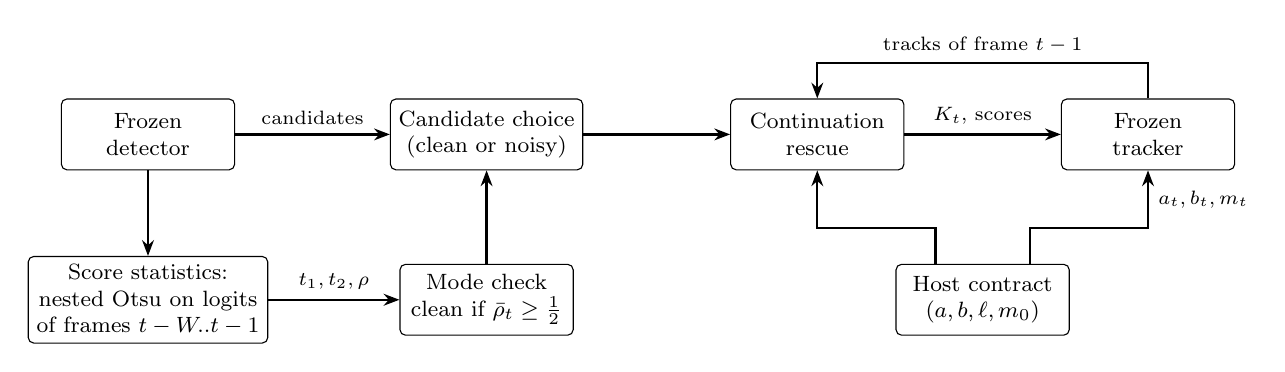
\begin{tikzpicture}[
  box/.style={draw, rounded corners=2pt, align=center, font=\footnotesize, minimum height=9mm, minimum width=22mm, inner sep=3pt},
  arr/.style={-{Stealth[length=2mm]}, thick}, lab/.style={font=\scriptsize}]
\node[box] (det) at (0,0) {Frozen\\detector};
\node[box] (pol) at (4.3,0) {Candidate choice\\(clean or noisy)};
\node[box] (res) at (8.5,0) {Continuation\\rescue};
\node[box] (trk) at (12.7,0) {Frozen\\tracker};
\node[box] (stat) at (0,-2.1) {Score statistics:\\nested Otsu on logits\\of frames $t-W..t-1$};
\node[box] (reg) at (4.3,-2.1) {Mode check\\clean if $\bar\rho_t \ge \tfrac12$};
\node[box] (hc) at (10.6,-2.1) {Host contract\\$(a, b, \ell, m_0)$};
\draw[arr] (det) -- node[lab, above]{candidates} (pol);
\draw[arr] (pol) -- (res);
\draw[arr] (res) -- node[lab, above]{$K_t$, scores} (trk);
\draw[arr] (det) -- (stat);
\draw[arr] (stat) -- node[lab, above]{$t_1, t_2, \rho$} (reg);
\draw[arr] (reg) -- (pol);
\draw[arr] (hc.north) ++(-0.6,0) |- ++(0,0.45) -| (res.south);
\draw[arr] (hc.north) ++(0.6,0) |- ++(0,0.45) -| node[lab, pos=0.75, right]{$a_t, b_t, m_t$} (trk.south);
\draw[arr] (trk.north) -- ++(0,0.45) -| node[lab, pos=0.25, above]{tracks of frame $t-1$} (res.north);
\end{tikzpicture}}
\caption{\scl{} between a frozen detector
and a frozen tracker. The statistics use earlier frames only. The host
contract holds the tracker's published settings. The tracker receives the
chosen candidates, their scores, and its thresholds for the frame.}
\label{fig:arch}
\end{figure*}

\subsection{Inputs and outputs}\label{sec:problem}
In each frame $t$, the detector gives a list of candidates
$D_t=\{(\mathbf{x}_i,s_i,c_i)\}$: a box $\mathbf{x}_i$, a score
$s_i\in(0,1)$, and a class label $c_i$ for each one, down to a lowest score
called the emission floor. The layer does not use the score itself but its
logit (log-odds), which spreads out scores close to 0 and 1:
\begin{equation}
z_i=\log\frac{s_i}{1-s_i}.
\label{eq:logit}
\end{equation}
For example, a score of 0.5 gives $z_i=0$, a score of 0.9 gives
$z_i\approx2.2$, and a score of 0.1 gives $z_i\approx-2.2$. The logistic
function $\sigma(z)=1/(1+e^{-z})$ turns a logit back into a score. Table~\ref{tab:symbols}
lists all symbols of the method.

The tracker, called the host, gives the layer four numbers about itself, the
host contract $h=(a,b,\ell,m_0)$. These are simply the settings that its
authors published: $a$ is the score a detection needs to be matched to a
track in the first step, $b$ is the score it needs to start a new track,
$\ell$ is the lowest score the tracker uses at all, and $m_0$ is its matching
tolerance (one minus the smallest overlap that still counts as a match). A
single-stage tracker uses one threshold, so $\ell=\min(a,b)$. A two-stage
tracker also uses weaker detections in a second step, so
$\ell<\min(a,b)$.

In every frame the layer returns five things: the candidates $K_t$ that the
tracker will see, their scores $\tilde{s}$, and the thresholds $(a_t,b_t)$
and tolerance $m_t$ that the tracker will use in this frame:
\begin{equation}
\left(K_t,\tilde{s},a_t,b_t,m_t\right)=
\mathcal{L}\left(Z_{<t},D_t,\mathcal{T}_{t-1},g_t;\,h\right).
\label{eq:layer}
\end{equation}
Here $Z_{<t}$ are the logits of the earlier frames, $\mathcal{T}_{t-1}$ are
the tracks of the previous frame, and $g_t$ is an optional measure of camera
motion in frame $t$. In words, Eq.~\eqref{eq:layer} says that the output for
frame $t$ depends only on the logits of earlier frames, the candidates of
frame $t$, the tracks of frame $t-1$, the camera motion, and the tracker's
contract. The decision for frame $t$ uses only past frames; frame $t$ is
added to the statistics after the decision, and no future frame is ever
used.

\begin{table}[t]
\caption{Main symbols of the method.}
\label{tab:symbols}
\centering\footnotesize
\begin{tabular}{@{}l>{\raggedright\arraybackslash}p{58mm}@{}}
\toprule
Symbol & Meaning\\
\midrule
$t$ & frame index\\
$D_t$ & candidates of frame $t$ given by the detector\\
$\mathbf{x}_i, s_i, c_i$ & box, score, and class label of candidate $i$\\
$z_i$ & logit (log-odds) of the score $s_i$, Eq.~\eqref{eq:logit}\\
$\sigma(\cdot)$ & logistic function, turns a logit back into a score\\
$h=(a,b,\ell,m_0)$ & host contract: the tracker's published settings\\
$a$, $b$ & score needed to match a track, and to start a new track\\
$\ell$ & lowest score the tracker uses\\
$m_0$ & matching tolerance: one minus the smallest IoU that counts as a match\\
$W$ & number of past frames used for the statistics (10)\\
$t_1$, $t_2$ & first and second Otsu split on the logits\\
$\rho_t$, $\bar\rho_t$ & share of confident candidates in frame $t$, and its median so far\\
$u_i$ & rank of candidate $i$ in the remap memory, from 0 to 1\\
$K_t$, $\tilde{s}$ & candidates passed to the tracker, and their scores\\
$a_t$, $b_t$, $m_t$ & thresholds and tolerance used by the tracker in frame $t$\\
$\mathcal{T}_{t-1}$ & tracks of the previous frame\\
$g_t$, $r_t$ & camera motion in frame $t$, and its ratio to the usual motion\\
IoU & intersection over union: overlap of two boxes, from 0 to 1\\
\bottomrule
\end{tabular}
\end{table}

Four goals guided the design. The layer needs no training and no labels. One
frozen configuration must work for every tracker, detector, and dataset.
When the tracker already fits the detector, its input must stay the same.
And the layer must take little time compared with the detector.

\subsection{Self-calibration from detector scores}\label{sec:calib}
A detector that suits the scene gives many low scores to background and a
separate group of high scores to objects. The layer checks, without labels,
how clearly this happens. It collects the logits of the candidates of the
last $W=10$ frames that remain after duplicate removal
(Sect.~\ref{sec:regimes}) and splits them twice with Otsu's method \cite{otsu1979},
which finds the threshold that best separates a histogram into two groups.
The first split, $t_1$, separates background from foreground. The second
split, $t_2$, divides the foreground into uncertain and confident candidates.
The share of confident candidates in the foreground,
\begin{equation}
\rho_t=\frac{\left|\{i: z_i\ge t_2\}\right|}{\left|\{i: z_i\ge t_1\}\right|},
\label{eq:rho}
\end{equation}
shows how clearly the detector separates objects from clutter. In words,
$\rho_t$ is the number of confident candidates divided by the number of
foreground candidates. For example, if 40 candidates are in the foreground
and 30 of them are confident, then $\rho_t=0.75$. A high $\rho_t$ means that most foreground candidates are confident; a low $\rho_t$
means that many of them are uncertain. Because the splits are made on
logits, they move with the scores when the whole logit scale is stretched or
shifted, for example by a change of temperature, and each group keeps the
same candidates.

These groups only make sense if there is a real background group. Some
detectors give very few low scores; then the first split falls inside the
objects. The layer detects this case, when fewer candidates lie below $t_1$
than above it, and counts the frame as clean, $\rho_t=1$. This background
check was added after a case seen during development: at the start of some
sequences, with about ten candidates per frame, the splits fell at
$t_1\approx0.6$ and $t_2\approx0.93$ in probability terms and gave a wrong
noisy decision.

\subsection{Clean and noisy modes}\label{sec:regimes}
The mode decides how much the layer may change. A clean stream means that
the detector already separates objects from clutter, so the tracker's own
settings are kept. A noisy stream means that many candidates are uncertain,
so the layer takes over the choice of candidates and thresholds.

\emph{Choosing the mode.} The stream is clean at frame $t$ if the median
$\bar\rho_t$ of all $\rho$ values so far (ignoring cold frames) is at least
one half, and noisy otherwise. Before the first valid split, for example in
the first frame, the mode is called cold. Because the median covers the whole
stream so far, the mode describes the detector and the scene, and a short
drop in confidence, for example during fast camera motion, does not change
it.

\emph{Cold and clean modes.} The tracker keeps its own thresholds. In the
clean mode there is one exception: if a threshold is so high that it would
reject the confident group, it is lowered to $t_2$:
\begin{equation}
a_t=\min\!\left(a,\sigma(t_2)\right),\qquad b_t=\min\!\left(b,\sigma(t_2)\right),
\label{eq:clean}
\end{equation}
where $\sigma$ is the logistic function, which turns a logit back into a
score. In words, each threshold stays as the tracker set it, unless it is
higher than the score $\sigma(t_2)$ at which the confident group begins; then
it is lowered to that score. Scores are passed unchanged, and only cross-class duplicates (one box
given two class labels) are removed. When the confident group already lies
above the tracker's thresholds, the tracker therefore receives exactly its
normal input.

\emph{Example.} When the detector scores are halved, no score is above 0.5.
A tracker with $a=0.6$ and $b=0.7$, such as ByteTrack in its official setting
(Table~\ref{tab:contracts}), then receives no detection that can start a
track, so it never creates a track. The Otsu splits are computed from the
halved scores themselves, so they move with them. In the clean mode,
Eq.~\eqref{eq:clean} then lowers the tracker's thresholds to $\sigma(t_2)$,
and the confident candidates reach the tracker again. In the noisy mode, the
new scores below place them at or above the thresholds of 0.5.
Section~\ref{sec:shift} shows the measured effect.

\emph{Noisy mode.} Here the layer decides which candidates the tracker may
use, and for what. Confident candidates ($z\ge t_2$) may start and continue
tracks. Uncertain candidates ($t_1\le z<t_2$) may only continue existing
tracks. Background candidates ($z<t_1$) are dropped. Each score is replaced
by a new one based on its rank $u_i$ in a memory of earlier scores: the share
of memory scores below it, with equal scores counted as one half (a mid-rank
empirical distribution value from 0 to 1). The memory holds the scores left
after duplicate removal in the first frame and in every tenth frame after it,
and keeps the last 20 such frames. It is separate from the window of $W$
frames used for the statistics, and while it is still empty, the scores of the
current frame are used instead. The new score is
\begin{equation}
\tilde{s}_i=
\begin{cases}
0.5+0.5\,u_i, & z_i\ge t_2,\\
0.1+0.4\,u_i, & t_1\le z_i<t_2,
\end{cases}
\label{eq:remap}
\end{equation}
and the tracker's matching and birth thresholds are both set to 0.5,
$a_t=b_t=0.5$. In words, the lowest-ranked confident candidate gets 0.5 and
the highest-ranked one gets close to 1, while an uncertain candidate gets a
score between 0.1 and 0.5 in the same order. Confident candidates thus get
scores of 0.5 and above, and
uncertain ones get scores below 0.5, so they can only reach a tracker's
low-score step. Duplicates are removed with the help of the tracks: a weaker
candidate that overlaps a stronger one with an intersection over union (IoU)
above one half is removed, unless a different track of the previous frame
claims it. This keeps people who stand close together in a crowd.

\subsection{Track continuation and camera motion}\label{sec:rescue}
A tracker ignores every candidate below its lowest threshold, so a track can
be lost when its object gets low scores for a few frames. This matters most
for single-stage trackers, which have no low-score step. The rescue gives
such a candidate a second chance, but only when it clearly continues an
existing track. Three conditions must hold: the candidate is in the
foreground ($z\ge t_1$, or any candidate for a single-stage tracker when
there is no background group); it overlaps a track of the previous frame
with an IoU of at least one half; and no other usable candidate covers that
track. Also, the tracker must be unable to see the candidate with the
thresholds of this frame. The candidate is then passed with its score raised
just above the tracker's lowest threshold. For a two-stage tracker, this only
applies to candidates below its low threshold $\ell$. For a single-stage
tracker, it applies to candidates below the lowest threshold used in this
frame, so the rescue gives it the continuation step it lacks.

When the camera moves fast, a box moves more between two frames, and a fixed
overlap requirement can break a correct match. In noisy frames, and only when
a motion measure is available, the matching tolerance therefore grows with
the current camera motion; $r_t$ is the current motion divided by its median
over past frames. The motion is the shift between two consecutive grayscale
frames at quarter resolution, found by phase correlation
\cite{reddy1996phasecorr} and divided by the image diagonal. The tolerance is
\begin{equation}
m_t=\min\!\left(0.95,\;1-\frac{1-m_0}{\max(1,r_t)}\right).
\label{eq:motion}
\end{equation}
In words, when the camera moves no faster than usual ($r_t\le1$), the
tolerance stays at $m_0$. When the motion is twice its usual value
($r_t=2$), the gap $1-m_0$ is halved: with $m_0=0.8$, the tolerance becomes
0.9, so a match needs an IoU of only 0.1 instead of 0.2. The tolerance never
exceeds 0.95.

\subsection{Host contract and adapters}\label{sec:contract}
Table~\ref{tab:contracts} lists the contracts used in this paper. Each value
is taken from the tracker's published configuration; none is fitted. A small
adapter for each tracker family passes the layer's decision to the tracker:
the chosen candidates and their scores replace the detector output of the
frame, and the new thresholds and tolerance replace the tracker's own for
that frame. Where a tracker has no overlap gate (C-TWiX) or uses two views of
the detections (TrackTrack), the adapter passes only what the tracker exposes.
In TrackTrack's second view, a detection that matches a candidate with an
overlap of at least 0.97, the tracker's own rule, follows that candidate. Any step that the authors apply after tracking, such as
interpolation or offline linking, is kept. The rules and their constants are
the same for every tracker. A tracker enters only through its four contract
values, and the adapter only passes on the decision; it never makes one.

\begin{table*}[t]
\caption{Host contracts: the published settings of each tracker, as used by
the layer: association threshold $a$, birth threshold $b$, lowest used score
$\ell$, and matching tolerance $m_0$ (Sect.~\ref{sec:problem}). A single-stage tracker has $\ell\ge\min(a,b)$. For trackers without
an overlap gate, $m_0$ is declared but not passed to the tracker.}
\label{tab:contracts}
\centering\footnotesize
\setlength{\tabcolsep}{3pt}
\begin{tabular}{@{}>{\raggedright\arraybackslash}p{37mm}lcccc>{\raggedright\arraybackslash}p{29mm}@{}}
\toprule
Tracker (setting) & Type & $a$ & $b$ & $\ell$ & $m_0$ & Decision passed to\\
\midrule
ByteTrack (official MOT17) & two-stage & 0.6 & 0.7 & 0.1 & 0.8 & candidates, scores, thresholds\\
ByteTrack (library setting; KITTI, VisDrone) & two-stage & 0.25 & 0.25 & 0.1 & 0.8 & same\\
BoT-SORT (library setting; KITTI) & two-stage & 0.25 & 0.25 & 0.1 & 0.8 & same\\
SparseTrack & two-stage & 0.6 & 0.7 & 0.1 & 0.85 & same\\
BoostTrack & two-stage & 0.6 & 0.6 & 0.1 & 0.7 & same\\
Hybrid-SORT & two-stage & 0.6 & 0.6 & 0.1 & 0.75 & same\\
TrackTrack (DanceTrack) & two-stage & 0.6 & 0.6 & 0.1 & 0.8 & candidates, scores, $a$ and $b$; both detection views\\
OC-SORT & single-stage & 0.6 & 0.6 & 0.6 & 0.7 & candidates, scores, thresholds\\
PD-SORT & single-stage & 0.6 & 0.6 & 0.6 & 0.7 & same\\
C-TWiX (MOT17 / KITTI / DanceTrack) & single-stage & 0.5 & 0.7 / 0.5 / 0.9 & 0.5 & 0.8 & candidates, scores, $a$ and $b$ (no overlap gate)\\
\bottomrule
\end{tabular}
\end{table*}


\subsection{Fixed constants}\label{sec:constants}
Table~\ref{tab:constants} lists every constant of the layer; the same values
are used for every tracker, detector, and dataset. The thresholds $t_1$ and
$t_2$ are not constants: they are computed again in every frame. Each
constant has a simple origin. The overlap of one half for duplicates and
rescue follows MOT evaluation, where two boxes with IoU above 0.5 cannot both
match different objects. The score ranges of Eq.~\eqref{eq:remap} put the two
groups on the common thresholds of 0.5 (matching and birth) and 0.1 (low
score). The cap of 0.95 keeps a minimum overlap of 0.05 for every match. The
window, the motion history, and the remap memory are default values that were
kept fixed in all development stages.

\begin{table}[t]
\caption{Fixed constants of \scl{}.}
\label{tab:constants}
\centering\footnotesize
\begin{tabular}{@{}>{\raggedright\arraybackslash}p{39mm}>{\raggedright\arraybackslash}p{31mm}@{}}
\toprule
Constant & Value\\
\midrule
Statistics window $W$ & 10 frames\\
Mode rule & clean if median $\rho\ge0.5$ over non-cold frames so far\\
Background check & $\rho=1$ if fewer candidates below $t_1$ than above\\
Noisy score ranges & primary $[0.5,1)$, extension $[0.1,0.5)$\\
Noisy association and birth thresholds & 0.5\\
Remap memory & 20 frames, one every 10 frames\\
Duplicate and rescue IoU & 0.5\\
Rescued score & lowest used threshold $+\,0.001$\\
Motion cue & phase correlation, quarter resolution\\
Motion history, warm-up & 100, 5 frames\\
Tolerance cap & 0.95\\
\bottomrule
\end{tabular}
\end{table}

\subsection{Per-frame steps and cost}\label{sec:cost}
Algorithm~\ref{alg:layer} gives the steps for one frame. The work per frame
is small: the layer sorts the logits of at most $W$ frames for the two Otsu
splits, computes overlaps between candidates and with the tracks of the
previous frame, and, when motion is used, computes one phase correlation on a
quarter-resolution image. With $n$ candidates per frame and $k$ tracks, the
cost is $O(Wn\log(Wn)+n^2+nk)$ plus a fixed image cost. The three terms
come from sorting the logits of the window, comparing every pair of
candidates, and comparing every candidate with every track. The layer stores only
the logits of the last $W$ frames, the per-frame $\rho$ values, the remap
memory, and the last 100 motion values.

\begin{algorithm}[t]
\caption{\scl{} for frame $t$. The window holds the logits of frames
$t-W$ to $t-1$, so the decision for frame $t$ uses no future frame.}\label{alg:layer}
\begin{algorithmic}[1]
\Require candidates $D_t$, tracks $\mathcal{T}_{t-1}$, motion cue $g_t$, contract $(a,b,\ell,m_0)$, constants of Table~\ref{tab:constants}
\Ensure candidates $K_t$, scores $\tilde{s}$, thresholds $a_t,b_t$, tolerance $m_t$
\State $z_i\gets$ logit of $s_i$ for all $i$ \Comment{Eq.~\eqref{eq:logit}}
\If{no valid split exists} \Comment{e.g., first frame}
  \State mode $\gets$ cold; $(a_t,b_t)\gets(a,b)$
\Else
  \State $(t_1,t_2)\gets$ nested Otsu on the window \Comment{Sect.~\ref{sec:calib}}
  \State $\rho_t\gets$ Eq.~\eqref{eq:rho} with the background check
  \State mode $\gets$ clean if $\mathrm{median}(\rho)\ge0.5$, else noisy
\EndIf
\If{mode is cold or clean} \Comment{Sect.~\ref{sec:regimes}}
  \State remove cross-class duplicates; keep raw scores
  \If{clean} set $(a_t,b_t)$ by Eq.~\eqref{eq:clean}
  \EndIf
\Else \Comment{noisy mode}
  \State remove duplicates with track context
  \State drop $z<t_1$; remap scores by Eq.~\eqref{eq:remap}
  \State $a_t\gets0.5$; $b_t\gets0.5$
\EndIf
\State rescue continuations (not cold) \Comment{Sect.~\ref{sec:rescue}}
\State $m_t\gets$ Eq.~\eqref{eq:motion} if noisy, else $m_0$
\State pass $K_t$, $\tilde{s}$, $a_t$, $b_t$, $m_t$ to the tracker
\State add the logits left after duplicate removal to the window
\State add $g_t$ to the motion history
\State store the tracks of frame $t$ after the tracker update
\end{algorithmic}
\end{algorithm}

\section{Development of the Method}\label{sec:development}

\subsection{Starting point: always-on banding}\label{sec:prior}
\scl{} was developed from an earlier design of the same research program,
called always-on banding (\aob{}). \aob{} computed the same nested Otsu
groups but treated every stream as noisy. In every frame it applied the
groups, removed every weaker candidate that overlapped a stronger one with
IoU above one half, and assigned all candidates new scores by rank on fixed
ranges. It passed no candidate in the first frame. \aob{} was designed for
noisy detector streams, and it is the baseline of this section.

Table~\ref{tab:prior} compares \aob{} and \scl{} with the same strong
published trackers on MOT17 \cite{milan2016mot16}. \aob{} lowered the HOTA of
SparseTrack by 4.15 points and that of BoostTrack by 5.89 points online and
5.37 points with interpolation, all with intervals below zero. Two causes
were found. First, removing overlapping boxes as duplicates deleted people
hidden behind others in crowds. Second, the self-calibrated thresholds were
stricter than the trackers' own: for SparseTrack and online BoostTrack, FP
fell by 1,630 and 1,351, but FN rose by 4,955 and 6,167. On the same trackers, \scl{} changed HOTA by $+0.06$ for SparseTrack
and left both BoostTrack versions identical to the host.
Figure~\ref{fig:prior} shows the same comparison.

\emph{What this stage showed.} A layer that acts in every frame harms
trackers that already fit the detector: strong published trackers lost
between 4.15 and 5.89 HOTA points in all three settings. Such a layer cannot
be placed safely in front of an unknown tracker. The next steps therefore let
the layer decide from the scores whether to act at all.

\begin{table}[t]
\caption{Baseline comparison of the development stage on MOT17 val-half
(published YOLOX-X detections). Host: published tracker alone (our
reproduction). $\Delta$: tracker with the earlier design \aob{} or with \scl{}
minus host, with 95\% paired-bootstrap interval (10,000 resamples,
seed 42). Bold intervals exclude zero.}
\label{tab:prior}
\centering\footnotesize
\setlength{\tabcolsep}{3pt}
\renewcommand{\arraystretch}{1.1}
\begin{tabular}{@{}lrcc@{}}
\toprule
Metric & Host & $\Delta$ \aob{} & $\Delta$ \scl{}\\
\midrule
\multicolumn{4}{@{}l}{\textit{SparseTrack} \cite{liu2025sparsetrack}}\\
\quad HOTA & 68.88 & \cibt{-4.15}{-5.54}{-1.66} & \cit{+0.06}{-0.01}{+0.25}\\
\quad MOTA & 77.85 & \cibt{-6.14}{-8.10}{-2.74} & \cit{+0.08}{-0.03}{+0.30}\\
\quad IDF1 & 81.97 & \cibt{-4.49}{-6.19}{-1.96} & \cit{+0.16}{-0.02}{+0.70}\\
\multicolumn{4}{@{}l}{\textit{BoostTrack, online} \cite{stanojevic2024boosttrack}}\\
\quad HOTA & 68.49 & \cibt{-5.89}{-7.76}{-2.87} & 0 (identical)\\
\quad MOTA & 75.50 & \cibt{-8.87}{-12.37}{-7.14} & 0 (identical)\\
\quad IDF1 & 81.41 & \cibt{-6.22}{-9.33}{-2.85} & 0 (identical)\\
\multicolumn{4}{@{}l}{\textit{BoostTrack, with interpolation} \cite{stanojevic2024boosttrack}}\\
\quad HOTA & 71.72 & \cibt{-5.37}{-7.30}{-2.75} & 0 (identical)\\
\quad MOTA & 81.03 & \cibt{-8.73}{-12.59}{-6.50} & 0 (identical)\\
\quad IDF1 & 84.16 & \cibt{-5.65}{-8.96}{-2.77} & 0 (identical)\\
\bottomrule
\end{tabular}
\end{table}


\begin{figure}[t]
\centering
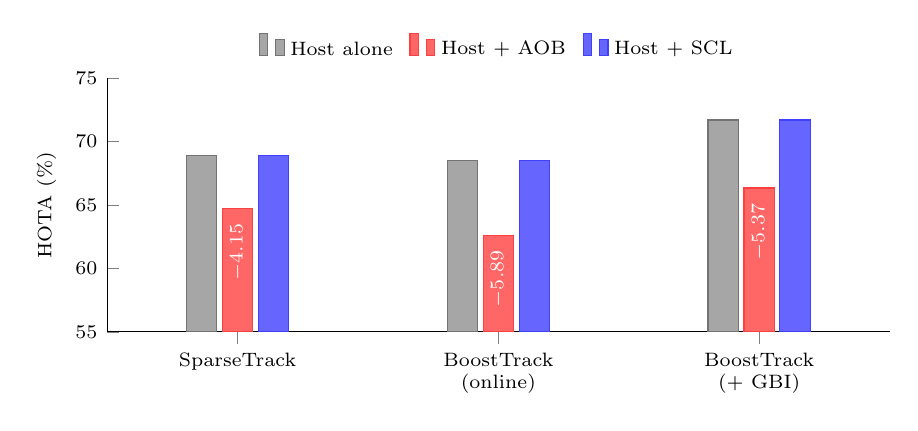
\begin{tikzpicture}
\begin{axis}[
  ybar,
  /pgf/bar width=11pt,
  width=0.95\columnwidth,
  height=4.8cm,
  ymin=55, ymax=75,
  xmin=0.5, xmax=3.5,
  xtick={1,2,3},
  xticklabels={SparseTrack, {BoostTrack\\(online)}, {BoostTrack\\(+ GBI)}},
  xticklabel style={align=center},
  ylabel={HOTA (\%)},
  axis x line*=bottom,
  axis y line*=left,
  tick label style={font=\scriptsize},
  label style={font=\scriptsize},
  legend style={at={(0.5,1.03)}, anchor=south, legend columns=3,
    font=\scriptsize, draw=none, /tikz/every even column/.append style={column sep=4pt}},
  legend cell align=left,
]
\addplot[fill=black!35, draw=black!55] coordinates {(1,68.88) (2,68.49) (3,71.72)};
\addplot[fill=red!60, draw=red!75] coordinates {(1,64.72) (2,62.61) (3,66.35)};
\addplot[fill=blue!60, draw=blue!75] coordinates {(1,68.93) (2,68.49) (3,71.72)};
\legend{Host alone, Host + \aob{}, Host + \scl{}}
\node[rotate=90, anchor=east, font=\scriptsize, text=white] at (axis cs:1,64.3) {$-4.15$};
\node[rotate=90, anchor=east, font=\scriptsize, text=white] at (axis cs:2,62.2) {$-5.89$};
\node[rotate=90, anchor=east, font=\scriptsize, text=white] at (axis cs:3,65.9) {$-5.37$};
\end{axis}
\end{tikzpicture}

\caption{HOTA on MOT17 val-half of strong published trackers (SparseTrack and
BoostTrack in two settings) alone, with \aob{}, and with \scl{}. The labels
give the change caused by \aob{}.}
\label{fig:prior}
\end{figure}

\subsection{Design steps}\label{sec:steps}
Each step from \aob{} to \scl{} was made to remove one cause found before it,
and it was compared with the step before it on development data
(Table~\ref{tab:ablation}). The steps, in the order in which they were made,
were the following.
\begin{itemize}
\item \emph{Starting point.} Running \aob{} inside the new framework showed
      the same problem: it reduced ByteTrack at floor 0.1 from 67.70 to 56.41
      HOTA and OC-SORT from 66.44 to 45.72.
\item \emph{Mode gate.} The two causes found in Sect.~\ref{sec:prior} were
      thresholds stricter than the trackers' own and the removal of hidden
      people as duplicates. The mode gate adds the mode check, the clean mode
      that keeps the tracker's settings, and the crowd-safe duplicate rule. It
      restored SparseTrack from 64.72 to 68.93 and BoostTrack from 62.61
      to 68.37.
\item \emph{Whole-stream mode.} The mode still changed in the middle of some
      streams. Choosing it from the whole stream removed these changes and
      raised ByteTrack from 67.561 to 67.702 and OC-SORT from 65.697 to
      66.071.
\item \emph{Continuation rescue.} Single-stage trackers still lost tracks
      whose objects got low scores for a few frames. The rescue added 0.2 to
      0.4 points for OC-SORT.
\item \emph{Background check.} A stream with few low-score candidates gave a
      wrong noisy decision (Sect.~\ref{sec:calib}). The background check
      completed \scl{}: it returned ByteTrack and BoostTrack to output
      identical to the host and raised OC-SORT to 67.04 and 66.91 at the two
      floors.
\end{itemize}
Four other versions were tested and rejected, because they lowered HOTA,
added FP, or let false tracks through on a noisy stream.

\emph{What this stage showed.} After these steps, the layer kept the strong
two-stage trackers at their own accuracy and improved the single-stage
OC-SORT. This is the behavior that the frozen configuration was then tested
for on new trackers, detectors, and data (Sect.~\ref{sec:results}).

\begin{table*}[t]
\caption{Design steps from \aob{} to \scl{} on development
data (HOTA, \%), and versions that were tested and rejected. The floor of
ByteTrack and OC-SORT is given in parentheses.}
\label{tab:ablation}
\centering\footnotesize
\setlength{\tabcolsep}{4pt}
\begin{tabular}{@{}>{\raggedright\arraybackslash}p{27mm}>{\raggedright\arraybackslash}p{37mm}>{\raggedright\arraybackslash}p{60mm}@{}}
\toprule
Step & Change & Effect\\
\midrule
\aob{} emulated & always-noisy bands, overlap deduplication, rank remap & ByteTrack (0.1) 56.41 vs host 67.70; OC-SORT (0.1) 45.72 vs 66.44\\
+ mode gate & mode statistic, host-anchored clean mode, crowd-safe duplicates & SparseTrack 64.72 to 68.93 (host 68.88); BoostTrack 62.61 to 68.37 (host 68.49)\\
+ whole-stream mode & mode from all past frames & ByteTrack (0.1) 67.561 to 67.702; OC-SORT (0.1) 65.697 to 66.071\\
+ continuation rescue & foreground track-consistent rescue & OC-SORT (0.01) 66.405 to 66.619; OC-SORT (0.1) 66.071 to 66.469\\
+ background check = \scl{} & no background mode gives no evidence against the host & ByteTrack/BoostTrack (0.1) identical to host; OC-SORT 67.041 (0.01), 66.907 (0.1)\\
\midrule
\multicolumn{2}{@{}l}{\textit{Rejected version}} & \textit{Evidence}\\
\multicolumn{2}{@{}l}{no candidates at frame 1} & $-0.3$ to $-0.5$ HOTA on every MOT17 host\\
\multicolumn{2}{@{}l}{rescue below a two-stage host's low stage} & FP $+700$ to $+1000$, $-0.4$ to $-0.5$ HOTA\\
\multicolumn{2}{@{}l}{rank-remapped scores in clean frames} & ByteTrack $-0.2$ / $-1.6$ HOTA\\
\multicolumn{2}{@{}l}{host-clipped noisy primary band} & KITTI YOLOv8n ByteTrack $+1.4$ HOTA but uncontrolled false tracks on a noisy aerial stream (VisDrone val, RT-DETR-L: 26.9 vs 14.9 boxes/frame)\\
\bottomrule
\end{tabular}
\end{table*}


\subsection{Freezing and testing}\label{sec:freeze}
The final configuration was frozen before any external test. It was saved in
a version-control tag and protected by a lock file that holds cryptographic
hashes of the layer, its configuration, and the evaluation scripts. Every
later run checked the lock before running. Sixty-one automated tests check
that the layer uses no future data, that its state resets between sequences,
that clean streams pass through unchanged, that the output does not depend on
detector, tracker, or sequence names, that affine score changes leave the
groups unchanged where designed, and that the lock is intact.

\section{Experimental Setup}\label{sec:setup}

The experiments test three expectations from the design. A tracker that
already fits its detector should keep its accuracy. A tracker that does not
fit, because it has no continuation step or because the detector or its
score scale changed, should gain. Both should hold on trackers and data that
were not seen during design.

\label{sec:hosts}Nine published trackers serve as hosts: ByteTrack
\cite{zhang2022bytetrack}, BoT-SORT \cite{aharon2022botsort}, OC-SORT
\cite{cao2023ocsort}, SparseTrack \cite{liu2025sparsetrack}, BoostTrack
\cite{stanojevic2024boosttrack}, PD-SORT \cite{wang2025pdsort},
Hybrid-SORT \cite{yang2024hybridsort}, C-TWiX \cite{miah2025twix}, and
TrackTrack \cite{shim2025tracktrack}. Each host uses the authors' code and
published configuration, and its contract is given in
Table~\ref{tab:contracts}. A tenth system, TOPICTrack
\cite{cao2025topictrack}, was selected under the post-freeze protocol, but
its reproduction failed (67.54 against the authors' 69.6 HOTA on MOT17
val-half), so it is excluded from the analysis.

In every comparison the baseline is the host alone: the published tracker,
run by us with its published configuration and the same detections. The
second run adds the frozen \scl{} and changes nothing else. Both runs use the
same environment and the same detections. Where the authors report their own
numbers, these are listed next to our reproduction of the host. All tracking
runs used a CPU only, without a graphics processing unit (GPU).
Where this changed the numerical precision or the software environment of an
external system, the difference is given with its reproduction
(Sect.~\ref{sec:external}).

\section{Results}\label{sec:results}

Figure~\ref{fig:forest} shows the HOTA difference between each host with
\scl{} and the host alone for every tested cell. The next subsections give
the baseline comparison for each part of the evaluation, in the order of the
three expectations of Sect.~\ref{sec:setup}: well-matched trackers, trackers
that do not fit their detector, and systems not seen during design.

\begin{figure}[t]
\centering
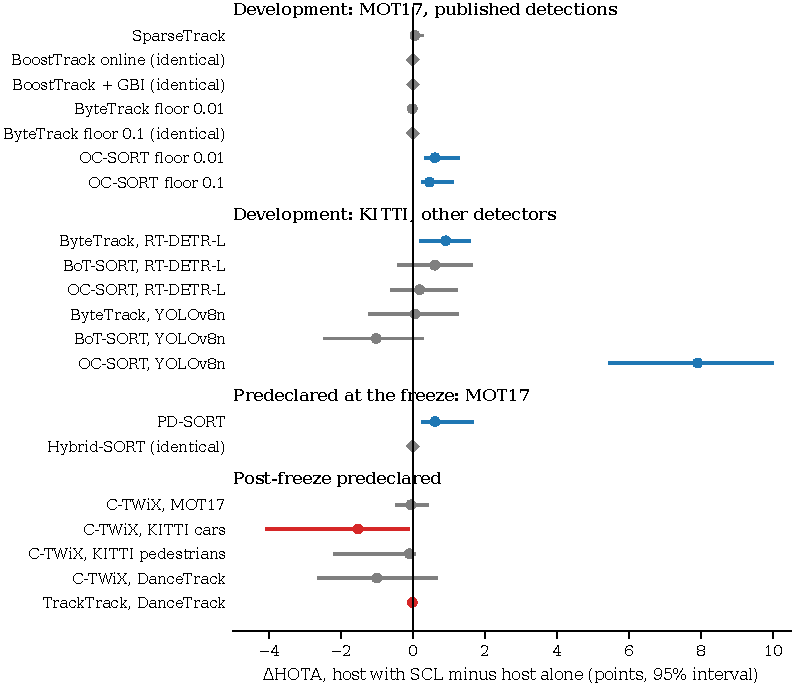
\includegraphics[width=0.82\textwidth]{figures/fig3_forest.pdf}
\caption{Difference in HOTA (host with \scl{} minus host alone) with
95\% paired-bootstrap interval for every tested cell. Blue: interval above
zero; red: interval below zero; gray: interval contains zero. Diamonds mark
identical output.}
\label{fig:forest}
\end{figure}

\subsection{Results across trackers}\label{sec:tracker}
Table~\ref{tab:mot17} compares the development trackers with their hosts on
MOT17. The two-stage trackers with well-matched detections stayed at the
accuracy of their hosts. BoostTrack, online and with interpolation, and
ByteTrack at floor 0.1 gave identical output. ByteTrack at floor 0.01
changed by $-0.014$ HOTA and SparseTrack by $+0.055$. This is the
self-limiting behavior of the clean mode (Sect.~\ref{sec:regimes}), which
the earlier design did not have (Table~\ref{tab:prior}).

The single-stage OC-SORT improved at both emission floors. Its HOTA rose by
0.61 points ($[+0.36,+1.24]$) at floor 0.01 and by 0.46 points
($[+0.27,+1.09]$) at floor 0.1, and its MOTA by 1.27 and 1.26 points. HOTA
was higher on 7 of 7 sequences in both settings (Fig.~\ref{fig:perseq}). The
gain comes from the continuation rescue. OC-SORT drops every detection
below its single threshold, and the layer passes it the foreground candidates
that continue a track that would otherwise stay unmatched.

\begin{table}[t]
\caption{Baseline comparison of the development trackers on MOT17 val-half
(published YOLOX-X detections). Paper: number reported by the tracker's
authors. Host: published tracker alone (our reproduction). $\Delta$: host with
\scl{} minus host, with 95\% paired-bootstrap interval (10,000
resamples, seed 42); bold intervals exclude zero. The floor is the lowest
detector score emitted.}
\label{tab:mot17}
\centering\footnotesize
\setlength{\tabcolsep}{4pt}
\begin{tabular}{@{}lrrl@{}}
\toprule
Metric & Paper & Host & $\Delta$ [95\% CI]\\
\midrule
\multicolumn{4}{@{}l}{\textit{SparseTrack} \cite{liu2025sparsetrack}}\\
\quad HOTA & 69.2 & 68.88 & $+0.06$ [$-0.01$, $+0.25$]\\
\quad MOTA & 76.8 & 77.85 & $+0.08$ [$-0.03$, $+0.30$]\\
\quad IDF1 & 81.4 & 81.97 & $+0.16$ [$-0.02$, $+0.70$]\\
\multicolumn{4}{@{}l}{\textit{BoostTrack, online} \cite{stanojevic2024boosttrack}}\\
\quad HOTA & 68.37 & 68.49 & 0 (identical)\\
\quad MOTA & 75.56 & 75.50 & 0 (identical)\\
\quad IDF1 & 81.35 & 81.41 & 0 (identical)\\
\multicolumn{4}{@{}l}{\textit{BoostTrack, + GBI} \cite{stanojevic2024boosttrack}}\\
\quad HOTA & 71.33 & 71.72 & 0 (identical)\\
\quad MOTA & 80.55 & 81.03 & 0 (identical)\\
\quad IDF1 & 83.84 & 84.16 & 0 (identical)\\
\multicolumn{4}{@{}l}{\textit{ByteTrack, floor 0.01} \cite{zhang2022bytetrack}}\\
\quad HOTA & -- & 67.70 & $-0.014$ [$-0.058$, $+0.009$]\\
\quad MOTA & 76.6 & 77.60 & $+0.06$ [$-0.15$, $+0.34$]\\
\quad IDF1 & 79.3 & 79.47 & $-0.031$ [$-0.135$, $+0.035$]\\
\multicolumn{4}{@{}l}{\textit{ByteTrack, floor 0.1} \cite{zhang2022bytetrack}}\\
\quad HOTA & -- & 67.70 & 0 (identical)\\
\quad MOTA & 76.6 & 77.60 & 0 (identical)\\
\quad IDF1 & 79.3 & 79.47 & 0 (identical)\\
\multicolumn{4}{@{}l}{\textit{OC-SORT, floor 0.01} \cite{cao2023ocsort}}\\
\quad HOTA & 66.5 & 66.43 & {\boldmath $+0.61$ [$+0.36$, $+1.24$]}\\
\quad MOTA & 74.9 & 74.67 & {\boldmath $+1.27$ [$+0.17$, $+3.01$]}\\
\quad IDF1 & 77.7 & 78.05 & $+0.66$ [$-0.25$, $+1.60$]\\
\multicolumn{4}{@{}l}{\textit{OC-SORT, floor 0.1} \cite{cao2023ocsort}}\\
\quad HOTA & 66.5 & 66.44 & {\boldmath $+0.46$ [$+0.27$, $+1.09$]}\\
\quad MOTA & 74.9 & 74.67 & {\boldmath $+1.26$ [$+0.37$, $+3.34$]}\\
\quad IDF1 & 77.7 & 78.05 & {\boldmath $+0.287$ [$+0.003$, $+0.838$]}\\
\bottomrule
\end{tabular}
\end{table}


\begin{figure}[t]
\centering
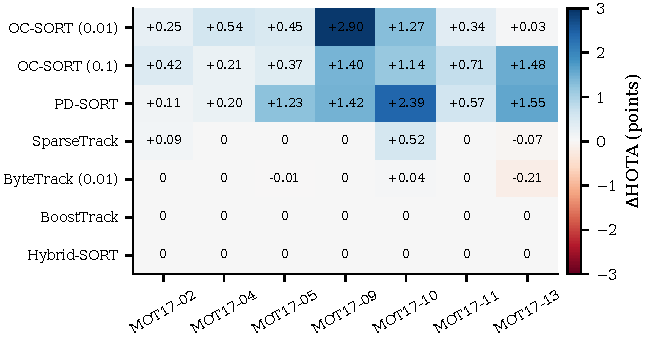
\includegraphics[width=0.75\textwidth]{figures/fig4_per_sequence.pdf}
\caption{Per-sequence HOTA differences (host with \scl{} minus host
alone) on MOT17 val-half for the development trackers and the external
trackers declared at the freeze.}
\label{fig:perseq}
\end{figure}

\subsection{Results with other detectors}\label{sec:detector}
Table~\ref{tab:kitti} reports all six KITTI cells: three trackers with each of
the two other detectors. With the noisy RT-DETR-L detector, the two-stage
trackers gained in MOTA and IDF1. ByteTrack gained 5.98 MOTA points
($[+1.16,+9.94]$), 3.87 IDF1 points, and 0.91 HOTA points
($[+0.22,+1.55]$). BoT-SORT gained 7.86 MOTA points ($[+2.21,+13.44]$) and
3.10 IDF1 points. OC-SORT with RT-DETR-L changed by less than 0.6 points in
every metric, with all intervals including zero. With YOLOv8n, the
single-stage OC-SORT gained 7.91 HOTA points ($[+5.47,+9.98]$), 9.40 MOTA
points, and 9.60 IDF1 points.

The two two-stage trackers with YOLOv8n are the regression case of the
development data. Their HOTA changed by $+0.06$ (ByteTrack) and $-1.02$
(BoT-SORT), both with intervals including zero, but their MOTA fell by 1.87
($[-6.25,+0.03]$) and 2.43 points ($[-7.43,-0.14]$), while identity switches
fell by 271 and 227, about half of the hosts' own counts. YOLOv8n gives many
correct detections with low scores, so the layer classified these streams as
noisy and allowed new tracks only from the confident group. This restriction
cost MOTA while it reduced identity switches. The regression was known when
the configuration was frozen.

\begin{table}[t]
\caption{Baseline comparison under a detector change on KITTI tracking
training (official HOTA, car and pedestrian averaged), all six cells. Host:
published tracker alone with the same detections. $\Delta$: host with \scl{}
minus host, with 95\% paired-bootstrap interval; bold intervals exclude zero.
BoT-SORT uses 20 of the 21 sequences in both arms: on sequence 0020, the
BoT-SORT Kalman update failed with a numerical (Cholesky) error when it
received the layer's output, while the host alone ran normally. This failure
case is excluded from both arms.}
\label{tab:kitti}
\centering\footnotesize
\setlength{\tabcolsep}{4pt}
\begin{tabular}{@{}lrlrl@{}}
\toprule
 & \multicolumn{2}{c}{RT-DETR-L} & \multicolumn{2}{c}{YOLOv8n}\\
\cmidrule(lr){2-3}\cmidrule(l){4-5}
Metric & Host & $\Delta$ [95\% CI] & Host & $\Delta$ [95\% CI]\\
\midrule
\multicolumn{5}{@{}l}{\textit{ByteTrack} \cite{zhang2022bytetrack}\textit{, library setting}}\\
\quad HOTA & 50.73 & {\boldmath $+0.91$ [$+0.22$, $+1.55$]} & 45.31 & $+0.06$ [$-1.19$, $+1.24$]\\
\quad MOTA & 47.27 & {\boldmath $+5.98$ [$+1.16$, $+9.94$]} & 46.54 & $-1.87$ [$-6.25$, $+0.03$]\\
\quad IDF1 & 64.98 & {\boldmath $+3.87$ [$+1.67$, $+5.06$]} & 60.92 & $+1.49$ [$-0.36$, $+3.27$]\\
\multicolumn{5}{@{}l}{\textit{BoT-SORT} \cite{aharon2022botsort}\textit{, library setting (20 sequences)}}\\
\quad HOTA & 53.91 & $+0.61$ [$-0.39$, $+1.61$] & 49.21 & $-1.02$ [$-2.43$, $+0.25$]\\
\quad MOTA & 48.25 & {\boldmath $+7.86$ [$+2.21$, $+13.44$]} & 49.89 & {\boldmath $-2.43$ [$-7.43$, $-0.14$]}\\
\quad IDF1 & 67.74 & {\boldmath $+3.10$ [$+1.00$, $+4.57$]} & 64.41 & $+0.35$ [$-2.10$, $+2.27$]\\
\multicolumn{5}{@{}l}{\textit{OC-SORT} \cite{cao2023ocsort}}\\
\quad HOTA & 52.64 & $+0.19$ [$-0.57$, $+1.19$] & 36.27 & {\boldmath $+7.91$ [$+5.47$, $+9.98$]}\\
\quad MOTA & 57.59 & $-0.57$ [$-4.36$, $+1.40$] & 33.99 & {\boldmath $+9.40$ [$+1.10$, $+12.30$]}\\
\quad IDF1 & 69.87 & $+0.04$ [$-1.31$, $+1.78$] & 50.46 & {\boldmath $+9.60$ [$+5.61$, $+12.16$]}\\
\bottomrule
\end{tabular}
\end{table}


\subsection{Results under shifted detector scores}\label{sec:shift}
Table~\ref{tab:shift} and Fig.~\ref{fig:shift} show the trackers under the
four score transforms. Halving the scores reduced ByteTrack (official setting)
and OC-SORT to 0 HOTA, because no detection reached their thresholds. With the
layer they reached 66.17 and 66.72. Cubing reduced them to 60.92 and 58.34,
and the layer restored them to 65.81 and 66.60. BoostTrack rose from 61.33 to
64.84 under cubing. With temperature $T=2$, the layer raised ByteTrack and
OC-SORT by 1.11 and 1.24 points. The library setting of ByteTrack, whose low
thresholds already accept the changed scores, stayed within 0.14 points in all
four transforms. Over the 14 conditions, the layer raised HOTA significantly
in 7 and lowered it significantly in none.

\begin{table}[t]
\caption{Baseline comparison under shifted detector scores on MOT17 val-half
(HOTA). The detector scores are transformed before the tracker, whose
published thresholds stay fixed; $T$ is a logit temperature, $\sigma(z/T)$.
Host: published tracker alone. $\Delta$: with \scl{} minus host,
with 95\% paired-bootstrap interval (10,000 resamples, seed 42). Bold
intervals exclude zero. Emission floor 0.01 (BoostTrack 0.1).}
\label{tab:shift}
\centering\footnotesize
\setlength{\tabcolsep}{4pt}
\begin{tabular}{@{}lrrl@{}}
\toprule
Transform & Host & + \scl{} & $\Delta$HOTA\\
\midrule
\multicolumn{4}{@{}l}{\textit{ByteTrack, official setting} \cite{zhang2022bytetrack}}\\
\quad $s^3$ & 60.92 & 65.81 & {\boldmath $+4.89$ [$+2.60$, $+13.69$]}\\
\quad $0.5\,s$ & 0.00 & 66.17 & {\boldmath $+66.17$ [$+49.32$, $+75.40$]}\\
\quad $T=2$ & 65.84 & 66.95 & {\boldmath $+1.11$ [$+0.35$, $+3.87$]}\\
\quad $T=0.5$ & 67.30 & 67.29 & $-0.009$ [$-0.051$, $+0.005$]\\
\multicolumn{4}{@{}l}{\textit{ByteTrack, library setting} \cite{zhang2022bytetrack}}\\
\quad $s^3$ & 66.31 & 66.31 & $-0.006$ [$-0.384$, $+0.383$]\\
\quad $0.5\,s$ & 66.61 & 66.48 & $-0.14$ [$-0.66$, $+0.14$]\\
\quad $T=2$ & 63.97 & 63.97 & 0 (identical)\\
\quad $T=0.5$ & 66.53 & 66.52 & $-0.006$ [$-0.029$, $+0.001$]\\
\multicolumn{4}{@{}l}{\textit{OC-SORT} \cite{cao2023ocsort}}\\
\quad $s^3$ & 58.34 & 66.60 & {\boldmath $+8.26$ [$+5.86$, $+16.81$]}\\
\quad $0.5\,s$ & 0.00 & 66.72 & {\boldmath $+66.72$ [$+50.32$, $+75.56$]}\\
\quad $T=2$ & 65.99 & 67.22 & {\boldmath $+1.24$ [$+0.52$, $+3.42$]}\\
\quad $T=0.5$ & 66.61 & 67.06 & $+0.45$ [$-0.01$, $+0.97$]\\
\multicolumn{4}{@{}l}{\textit{BoostTrack, online} \cite{stanojevic2024boosttrack}}\\
\quad $s^3$ & 61.33 & 64.84 & {\boldmath $+3.51$ [$+0.85$, $+13.28$]}\\
\quad $T=2$ & 67.59 & 67.59 & 0 (identical)\\
\bottomrule
\end{tabular}
\end{table}


\begin{figure}[t]
\centering
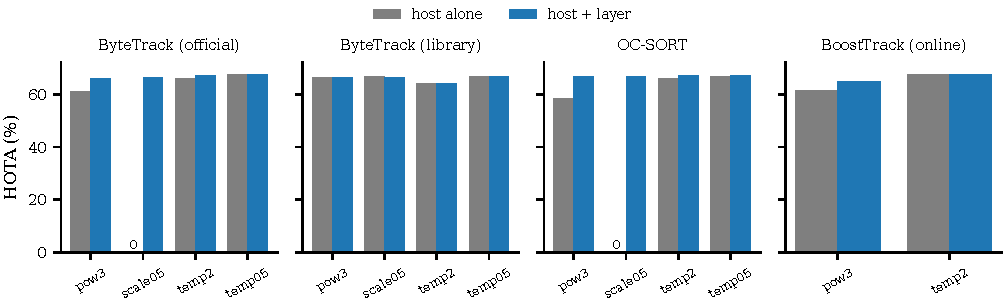
\includegraphics[width=\textwidth]{figures/fig5_calibration_shift.pdf}
\caption{Shifted detector scores on MOT17 val-half: HOTA of each published
tracker with its published thresholds, alone and with \scl{}, after
four monotone transforms of the detector scores (pow3: $s^3$; scale05:
$0.5\,s$; temp2 and temp05: $T=2$ and $T=0.5$).}
\label{fig:shift}
\end{figure}

\subsection{Results on external trackers}\label{sec:external}
Table~\ref{tab:external} gives every external system that passed its
reproduction. The external tests use new trackers on public benchmarks, each
with the detections that its authors released, so they test the transfer of
the frozen configuration to trackers, and with C-TWiX and TrackTrack also to
other detectors and datasets; they do not use new data.

\emph{Declared at the freeze.} PD-SORT \cite{wang2025pdsort} was reproduced
exactly as in the authors' released output. With \scl{}, its HOTA rose by 0.61
points ($[+0.27,+1.65]$), its MOTA by 1.13 points ($[+0.27,+3.03]$), and its
IDF1 by 0.82 points ($[+0.43,+1.94]$), with higher HOTA on 7 of 7 sequences
(Fig.~\ref{fig:perseq}). FN fell by 1,291, and FP rose by 681. PD-SORT is a
single-stage tracker, and its gain comes from the same step as for OC-SORT;
unlike OC-SORT, it was not seen during design. Hybrid-SORT
\cite{yang2024hybridsort}, a two-stage tracker, gave identical output, as
predicted before the run. Its reproduction was 0.40 HOTA below the authors'
number (CLOSE). The likely causes are the half-precision detections released
by the authors, whereas their reported number used full-precision inference,
and the software environment; the cause was documented but not isolated.

\emph{Declared after the freeze.} C-TWiX \cite{miah2025twix}, a single-stage
tracker that learns association from box coordinates, was reproduced on three
datasets: exactly on KITTI cars (89.27 against 89.3 HOTA), and within the
CLOSE class on KITTI pedestrians (70.77 against 71.4), MOT17 (77.55 against
77.8), and DanceTrack (59.62 against 60.4). It ran with the authors'
half-precision setting, but on a CPU instead of a GPU. On MOT17 the layer changed its HOTA
by $-0.05$ ($[-0.46,+0.40]$), on KITTI pedestrians by $-0.10$
($[-2.16,+0.03]$), and on DanceTrack by $-1.00$ ($[-2.62,+0.65]$). On KITTI
cars it lowered HOTA by 1.52 points ($[-4.05,-0.13]$), the only significant
external HOTA loss larger than 0.1 points. TrackTrack \cite{shim2025tracktrack}, a
two-stage tracker, was reproduced within 0.34 HOTA on DanceTrack (CLOSE, with
full-precision appearance features on a CPU). The layer changed its HOTA by
$-0.013$ ($[-0.032,-0.001]$): the interval excludes zero, but the effect is
negligible, and 21 of 25 sequences were tied. TOPICTrack failed its
reproduction and is excluded (Sect.~\ref{sec:setup}); the layer's effect on it
($-0.016$ HOTA, interval including zero) was recorded but is not analyzed.

The protocol also fixed predictions before these runs. For C-TWiX on MOT17 it
predicted no loss in HOTA; the measured $-0.05$ is a small loss with an
interval including zero, so the prediction did not hold. For KITTI and
DanceTrack it predicted a change of less than one HOTA point; this held for
KITTI pedestrians but not for KITTI cars ($-1.52$) or DanceTrack ($-1.00$).
For TOPICTrack, a change of at most 0.1 points was predicted and observed,
but this system is excluded. Section~\ref{sec:discussion} analyzes the
C-TWiX losses.

\begin{table*}[t]
\caption{Baseline comparison on the external systems, each run once with the frozen \scl{}.
Top: declared at the freeze (MOT17 val-half, authors' released detections). Bottom:
declared after the freeze under the registered protocol (authors' released detections;
TrackTrack after its post-processing, as in its paper). Ref.: HOTA reported by the
authors (for PD-SORT, their released output). Class: reproduction against Ref. (EXACT:
$|\Delta\mathrm{HOTA}|\le0.2$; CLOSE: $\le1.0$ with a documented, untuned cause).
Host: HOTA of the published tracker alone (our reproduction). $\Delta$: host with \scl{}
minus host, with the 95\% paired-bootstrap interval below it; bold intervals exclude zero.
W/T/L: sequences where HOTA rose, stayed within 0.01, or fell; ped.: pedestrians. TOPICTrack (FAILED
reproduction) is excluded.}
\label{tab:external}
\centering\footnotesize
\setlength{\tabcolsep}{2.5pt}
\renewcommand{\arraystretch}{1.15}
\begin{tabular}{@{}llccccc@{}}
\toprule
System (class) & Data & \twol{Ref.}{Host} & $\Delta$HOTA & $\Delta$MOTA & $\Delta$IDF1 & W/T/L\\
\midrule
\twol{PD-SORT \cite{wang2025pdsort}}{(EXACT)} & MOT17 & \twol{68.01}{68.01} & \cib{+0.61}{+0.27}{+1.65} & \cib{+1.13}{+0.27}{+3.03} & \cib{+0.82}{+0.43}{+1.94} & 7/0/0\\
\twol{Hybrid-SORT \cite{yang2024hybridsort}}{(CLOSE)} & MOT17 & \twol{67.1}{66.70} & \twol{0}{(identical)} & 0 & 0 & 0/7/0\\
\midrule
\twol{C-TWiX \cite{miah2025twix}}{(CLOSE)} & MOT17 & \twol{77.8}{77.55} & \ci{-0.05}{-0.46}{+0.40} & \ci{+0.24}{-0.58}{+1.12} & \ci{+0.18}{-0.47}{+1.14} & 2/1/4\\
\twol{C-TWiX \cite{miah2025twix}}{(EXACT)} & KITTI cars & \twol{89.3}{89.27} & \cib{-1.52}{-4.05}{-0.13} & \cib{-2.11}{-5.89}{-0.17} & \cib{-1.21}{-3.32}{-0.10} & 2/2/5\\
\twol{C-TWiX \cite{miah2025twix}}{(CLOSE)} & KITTI ped. & \twol{71.4}{70.77} & \ci{-0.10}{-2.16}{+0.03} & \ci{-0.31}{-4.86}{+0.10} & \ci{-0.01}{-1.90}{+0.08} & 1/7/1\\
\twol{C-TWiX \cite{miah2025twix}}{(CLOSE)} & DanceTrack & \twol{60.4}{59.62} & \ci{-1.00}{-2.62}{+0.65} & \ci{+0.13}{-0.39}{+0.47} & \ci{-1.55}{-3.76}{+0.52} & 10/3/12\\
\twol{TrackTrack \cite{shim2025tracktrack}}{(CLOSE)} & DanceTrack & \twol{63.3}{62.96} & \cib{-0.013}{-0.032}{-0.001} & \cib{-0.073}{-0.208}{-0.004} & \ci{+0.009}{-0.001}{+0.028} & 0/21/4\\
\bottomrule
\end{tabular}
\end{table*}


\subsection{Summary over all cells}\label{sec:summary}
Of the 16 cells in Fig.~\ref{fig:forest} with an interval, 7 exclude zero in
HOTA: 5 above zero (OC-SORT twice on MOT17, OC-SORT with YOLOv8n and
ByteTrack with RT-DETR-L on KITTI, and PD-SORT) and 2 below (C-TWiX on KITTI
cars, $-1.52$, and TrackTrack, $-0.013$). Four further cells gave identical
output. In MOTA, the layer gave significant gains for OC-SORT on MOT17 and
with YOLOv8n, for PD-SORT, and for ByteTrack and BoT-SORT with RT-DETR-L, and
significant losses for BoT-SORT with YOLOv8n, C-TWiX on KITTI cars, and
TrackTrack. The external evidence is therefore mixed in sign and small in
size, except for the single-stage PD-SORT, the only external system whose
HOTA, MOTA, and IDF1 intervals are all above zero. With 7 to 25 sequences
per cell, the intervals are wide, and differences below a few tenths of a
HOTA point are not resolved unless the output is nearly identical.

\subsection{Running time}\label{sec:latency}
\label{sec:latency-setup}Running time was measured after the freeze on one cloud machine with a 4-vCPU
Intel Xeon processor at 2.10 GHz, 15 GB of memory, and no GPU. A live YOLOv8n
detector (32-bit floats, 736 pixels, batch 1) feeds ByteTrack on three KITTI
tracking sequences (0001, 0009, and 0019). Both runs use the same frames
one after the other, and the first ten frames of each sequence are excluded,
which leaves 2,279 timed frames per run. The time of the layer includes the
motion cue, the per-frame step, and saving the tracker output.

Table~\ref{tab:runtime} and Fig.~\ref{fig:runtime} compare the time per frame
of the host pipeline with and without \scl{}. \scl{} took 2.95 ms per
frame on average and 4.39 ms at the 95th percentile, including the
phase-correlation motion cue. The total time rose from 57.85 to 60.44 ms
per frame, by 4.5\%, so the whole pipeline ran at about 16.5 frames per second
on this CPU. The tracker became faster, from 2.04 to 1.43 ms per frame,
because it received fewer candidates. The detector takes most of each frame,
about 42 ms, so whether the full system runs in real time depends on the
detector and the hardware; the layer itself adds only a small part of the
total time.

\begin{table}[t]
\caption{Baseline comparison of the per-frame time on a 4-vCPU Intel Xeon
(2.10 GHz, no GPU) with a live YOLOv8n detector (736 pixels) and ByteTrack on
three KITTI sequences (2,279 timed frames per arm). Host alone: the same
pipeline without \scl{}. Mean / 95th percentile in milliseconds.}
\label{tab:runtime}
\centering\footnotesize
\setlength{\tabcolsep}{4pt}
\begin{tabular}{@{}lcc@{}}
\toprule
Stage & Host alone & Host + \scl{}\\
\midrule
Frame decode & 13.88 / 16.21 & 13.88 / 16.51\\
Detector (YOLOv8n, 736 px) & 41.91 / 58.41 & 42.17 / 59.43\\
\scl{} & -- & 2.95 / 4.39\\
Tracker (ByteTrack) & 2.04 / 3.57 & 1.43 / 2.64\\
End to end & 57.85 / 76.35 & 60.44 / 80.78\\
\bottomrule
\end{tabular}
\end{table}


\begin{figure}[t]
\centering
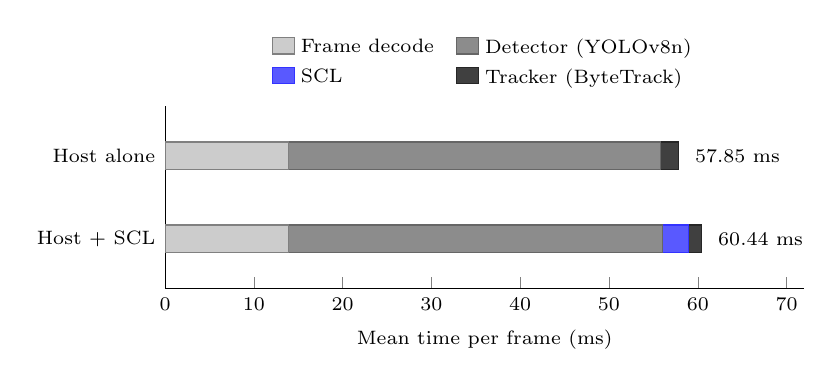
\begin{tikzpicture}
\begin{axis}[
  xbar stacked,
  /pgf/bar width=10pt,
  width=0.8\columnwidth,
  height=3.9cm,
  xmin=0, xmax=72,
  clip=false,
  ymin=-0.6, ymax=1.6,
  ytick={0,1},
  yticklabels={Host + \scl{}, Host alone},
  xlabel={Mean time per frame (ms)},
  axis x line*=bottom,
  axis y line*=left,
  tick label style={font=\scriptsize},
  label style={font=\scriptsize},
  legend style={at={(0.5,1.04)}, anchor=south, legend columns=2,
    font=\scriptsize, draw=none, /tikz/every even column/.append style={column sep=6pt}},
  legend cell align=left,
]
\addplot[fill=black!20, draw=black!50] coordinates {(13.88,1) (13.88,0)};
\addplot[fill=black!45, draw=black!60] coordinates {(41.91,1) (42.17,0)};
\addplot[fill=blue!65, draw=blue!80] coordinates {(0,1) (2.95,0)};
\addplot[fill=black!75, draw=black!85] coordinates {(2.04,1) (1.43,0)};
\legend{Frame decode, Detector (YOLOv8n), \scl{}, Tracker (ByteTrack)}
\node[anchor=west, font=\scriptsize] at (axis cs:58.6,1) {57.85 ms};
\node[anchor=west, font=\scriptsize] at (axis cs:61.2,0) {60.44 ms};
\end{axis}
\end{tikzpicture}

\caption{Mean per-frame time by stage for the host pipeline alone and with
\scl{} (4-vCPU Intel Xeon, no GPU). The labels give the measured
end-to-end time.}
\label{fig:runtime}
\end{figure}

\section{Discussion}\label{sec:discussion}

\emph{When the layer acts.} The effect depends on two properties of the
pipeline, not on the dataset: whether the tracker has a continuation step,
and whether the detector's scores match the tracker's thresholds. On MOT17
with well-matched detections, the two-stage trackers BoostTrack, ByteTrack at
floor 0.1, and Hybrid-SORT produced output identical to their hosts, while
the single-stage OC-SORT and PD-SORT gained HOTA on every sequence. On the
external streams declared after the freeze, the layer classified at least
99.7\% of the frames as clean on MOT17 and DanceTrack, and it left those
pipelines at or near their own output. When the stream fits the tracker, the
layer mostly stays out of the way, and when the tracker lacks a step, the
layer adds it.

\emph{Self-limiting by design.} In the clean mode the layer keeps the
tracker's thresholds and scores, so a tracker with a low-score step and
well-matched detections receives its normal input. This is the main
difference from the earlier design \aob{}, which lowered the HOTA of the same
strong trackers by 4.15 to 5.89 points (Table~\ref{tab:prior}). The layer
therefore does not need to know in advance whether a tracker needs help; it
reads the answer from the scores.

\emph{Detector replacement.} When a detector is replaced or its score scale
shifts, the fixed thresholds of a tracker no longer match the scores. The
layer adjusts them from the scores without labels. Under halved scores it
restored two trackers from 0 to about 66 HOTA, and with a different detector
it raised the MOTA of two two-stage trackers by 6.0 and 7.9 points. This is
the case the layer was built for: a detector that is swapped, retrained, or
quantized while the tracker stays the same.

\emph{Failure cases.} Three results go against the layer. First, with the
under-confident YOLOv8n detector on KITTI, the noisy mode restricted new
tracks of the two two-stage trackers and cost them 1.87 and 2.43 MOTA points
(Sect.~\ref{sec:detector}). Second, the loss of C-TWiX on KITTI cars
($-1.52$ HOTA) comes almost entirely from one short sequence: in sequence 0014
the layer classified 45 of 106 frames as noisy, and HOTA fell by 17.09 points,
while six of the other eight sequences changed by less than 0.4 points. The
same sequence causes the loss on KITTI pedestrians (8.50 points in that
sequence). In such a short sequence, the median of $\rho$ over the stream has
little history, and the restrictions of the noisy mode most likely removed
detections that the coordinate-based association of C-TWiX relies on; this
mechanism was not isolated further. A rule that requires a minimum history
before a noisy decision is a natural remedy, but it was not part of the frozen
configuration. Third, C-TWiX on DanceTrack lost 1.00 HOTA with an interval
including zero; two sequences lost more than 10 points and one gained 9.37.
The stream was clean on almost every frame, so the effect comes from the
operations of the clean mode (cross-class duplicate removal, threshold
lowering to $\sigma(t_2)$, and the continuation rescue) acting on a tracker
that learns association from coordinates; which of them causes the loss was
not isolated.

\emph{Limitations.} The strongest evidence is development evidence: the
configuration was selected on MOT17, KITTI, and VisDrone, so the gains there
are not held out. Only four external systems passed their reproduction, and
only PD-SORT improved. The external tests change the tracker, and with C-TWiX
and TrackTrack the detector and the dataset, but they use the detections
released by each tracker's authors on public benchmarks, not new data. The
paired intervals are computed for each comparison separately, without a
correction for multiple comparisons, and with 7 to 25 sequences per cell they
are wide. Finally, the layer was compared with each tracker alone and with
its own earlier design, not with other adaptive methods such as Adaptive
ByteTrack \cite{ma2023adaptivebytetrack} or ACT \cite{act2026adaptive}, nor
with a threshold-only or a rescue-only variant of itself; these comparisons
are left for future work.

\emph{Relation to detector-side control.} Our earlier AC-MOT controller,
described in a manuscript submitted for publication, acts before the detector
and chooses its operating point from the scene. \scl{} acts after the
detector and adapts the tracker's input to the scores that the detector
produces. The two layers work on different parts of the pipeline, so they
could be used together; combining them is left for future work.

\emph{Cost.} The layer needs no training, no GPU, and no access to the inside
of the detector, and it needs only four contract values from the tracker's
configuration. At run time it reads the candidate list, one small grayscale
image for the motion cue, and the tracks of the previous frame. On a CPU it
takes 2.95 ms per frame, adds 4.5\% to the total time of the tested pipeline,
and makes the tracker itself faster. New trackers are added through their
published contract values and an adapter, without changes to the rules.

\section{Conclusion}\label{sec:conclusion}

This paper presented \scl{}, a control layer that needs no training, adjusts
itself from a detector's scores, and adapts a frozen tracker through a
declared host contract. The layer splits the logits of recent frames with
nested Otsu thresholds and decides whether the stream is clean or noisy. On
clean streams it keeps the tracker's settings; on noisy streams it chooses
the candidates, assigns them new scores, and sets the thresholds. A
continuation rescue gives single-stage trackers the step they lack.

One frozen configuration, developed step by step from \aob{}, was tested with
nine published trackers on MOT17, KITTI, and DanceTrack. It improved
single-stage trackers and trackers whose detector or score scale had changed,
kept well-matched two-stage trackers within 0.1\% of their HOTA, and took 2.95
ms per frame on a CPU. It also lowered the MOTA of two two-stage trackers with
an under-confident detector and the HOTA of a coordinate-based tracker on one
short KITTI sequence, and all such cases are reported. These results support
placing a self-calibrating layer between the detector and the tracker in
systems where the detector changes while the tracker stays the same, with a
rule for short streams and comparisons with other adaptive methods as the next
steps.


\backmatter

\bmhead{Acknowledgements}
The authors thank the authors of the evaluated trackers for releasing their code, weights, and
detections, and the maintainers of MOT17, KITTI, DanceTrack, VisDrone, and TrackEval.
AI-assisted tools were used for language editing and LaTeX formatting; the authors are
responsible for all content.

\section*{Statements and Declarations}

\bmhead{Funding}
The authors did not receive support from any organization for the submitted work.

\bmhead{Competing interests}
The authors have no competing interests to declare that are relevant to the content of this
article.

\bmhead{Ethics approval and consent to participate}
Not applicable. The study uses only public benchmark datasets and involves no human participants
or animals.

\bmhead{Data availability}
The datasets analysed in this study are publicly available: MOT17
(\url{https://motchallenge.net}), KITTI tracking (\url{https://www.cvlibs.net/datasets/kitti}),
DanceTrack (\url{https://github.com/DanceTrack/DanceTrack}), and VisDrone2019-MOT
(\url{https://github.com/VisDrone/VisDrone-Dataset}). The detections released by the authors of the
evaluated trackers were obtained from their public repositories. The per-sequence results,
bootstrap outputs, and run logs generated in this study are available from the corresponding author
on reasonable request.

\bmhead{Code availability}
The code of the layer, its frozen configuration with the lock file of cryptographic hashes, the
tracker adapters, and the evaluation scripts are available from the corresponding author on
reasonable request.

\bmhead{Author contributions}
Ahmed Gouda Ismail: conceptualization, methodology, software, investigation, formal analysis, and
writing of the original draft. Mohamed S. Mohamed and Tarek Ahmed Mahmoud: supervision, and
review and editing of the manuscript. All authors read and approved the final manuscript.

\bibliography{references}

\end{document}
